\subsection{Test Journal: Evaporator component model} \label{app:tj_1}

\textbf{Executed by: Kasper} \\
\textbf{Date: 10/5/2022}

\subsubsection*{Objective}
This test aims to document the behavior of the evaporator model with two distinct changes/ versions that are implemented in a class, called evaporatorModel.

\subsubsection*{Background}
The evaporator component "evaporatorModel" has proven to give us problems regarding its performance and outputs when compared with the HiFi simulation model provided by BITZER.
It would be advantageous to have indications that all of the component models are working before proceeding to the collection of the components, and the evaporator has proven to be the hardest component to get acceptable results from.

\subsubsection*{Test subject}
The test subject is the class "evaporatorModel". It consists of the equations \cref{eq:Evaporator_boundary} to\cref{eq:evap_dMvdt}.
Because of a suspicion of the positive feedback between the specific volume and the output pressure and that the output pressure in the Hifi simulation proved to be almost equal to the input pressure, we wanted to try to set these equal to each other and test this.

\subsubsection*{Equipment used}
The outputs from a simulation of "eTRU\_prototype\_2\_old\_perhabs\_with\_measurements.slx" are used as inputs for the test. The imported data can be found in "HiFi\_model\_data\_for\_component\_tests\_03.mat".
The script used for the tests are to be found in "componentModelTesting.m". with support from testinit.m.
All the files can be found in the git repository under CA8Project/Modeling/ComponentSimulation with the commit hash feff043be9d98efef19ba4f0f4ad9552baca9bf1.

\subsubsection*{Test setup}


\subsubsection*{Test procedure}
In the evaporator model on line 158, the update of the output pressure is commented out as

\begin{figure}[h!]
	\centering
	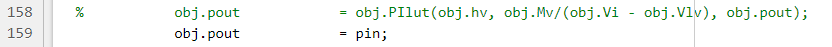
\includegraphics[width=0.7\textwidth]{Tests/Evapo_test1/pout_code.png}
	\caption{Code}
	\label{fig:evapotest1_code}
\end{figure}

now comment in 158 and comment out 159
and run the script "ComponentModelTesting.m". Now save the Figure 94.
Afterwards make sure the code in the evaporator model is reverted back to status in the above code, and run the script again and save the plot in Figure 94


\subsubsection*{Results and Comments}
First comes two plots with the output pressure being as in line 158 in \cref{fig:evapotest1_code}, \cref{fig:evapotest_plot1} showing the simulation with a start around time t= 2637 s and to the end.

\begin{figure}[h]
	\centering
	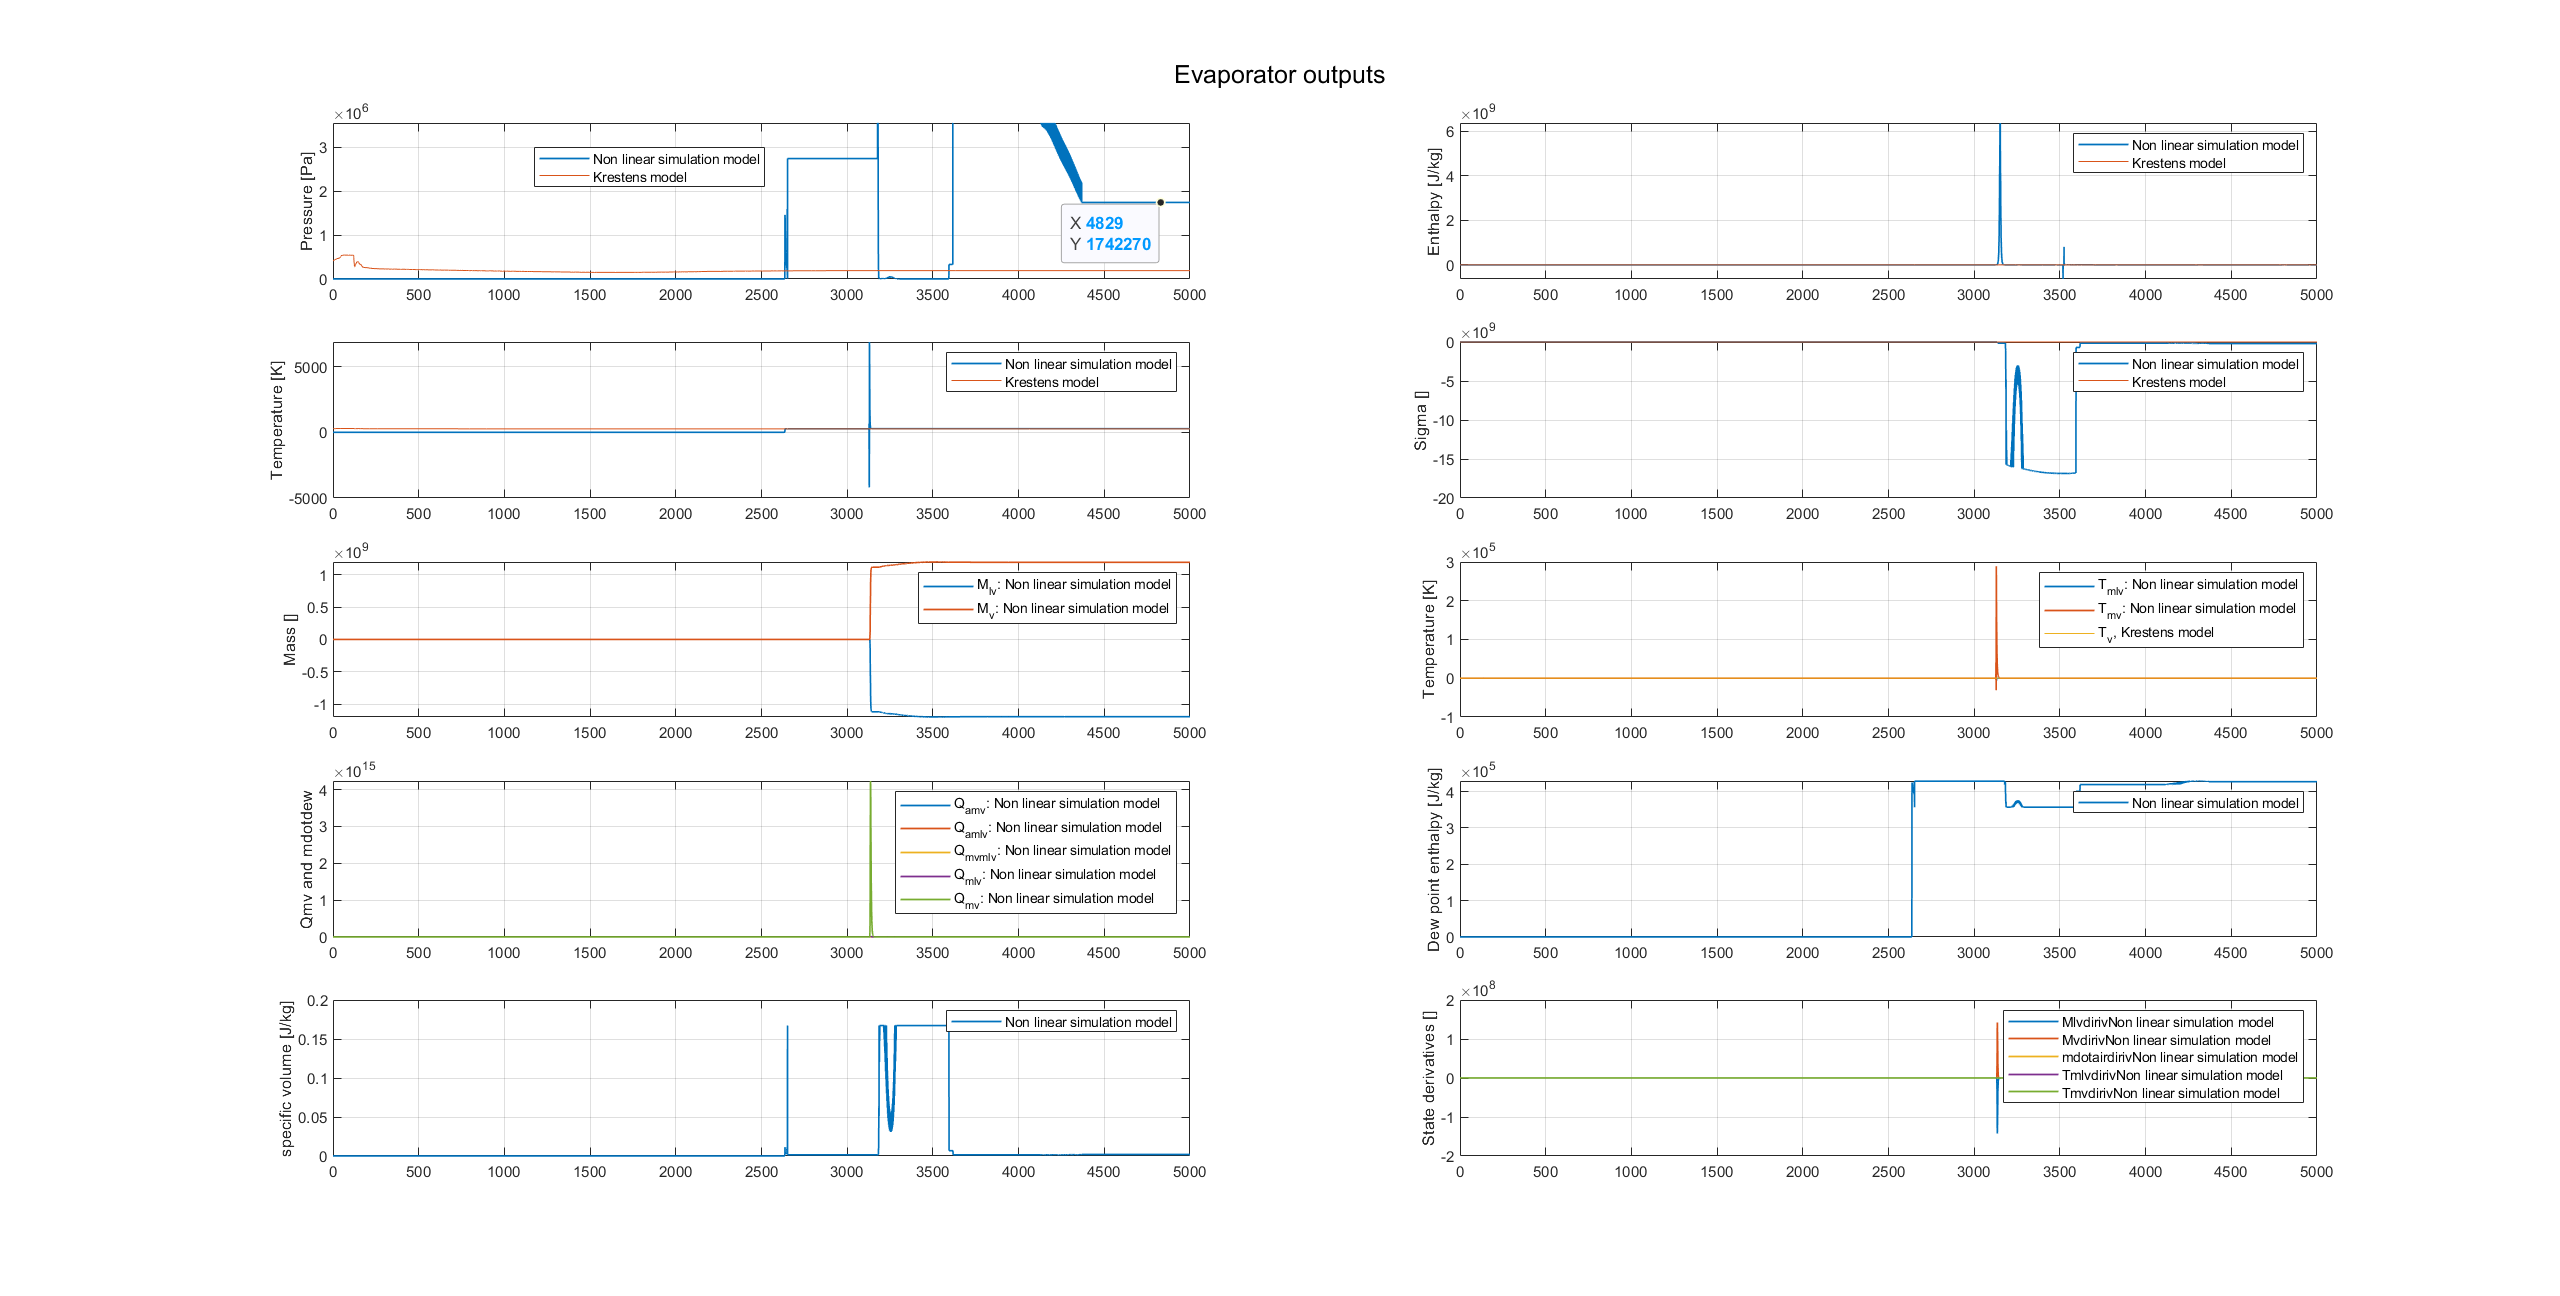
\includegraphics[width=2.1\textwidth]{Tests/Evapo_test1/plot_unstable.png}
	\caption{Outputs with pressure out being a table lookup}
	\label{fig:evapotest_plot1}
\end{figure}

Here if the upper left plot is observed, the output pressure of the evaporator model shows unstable behavior and eventual settling around a way to high value of 17.4 bar = 1740000 Pa.

\begin{figure}[h]
	\centering
	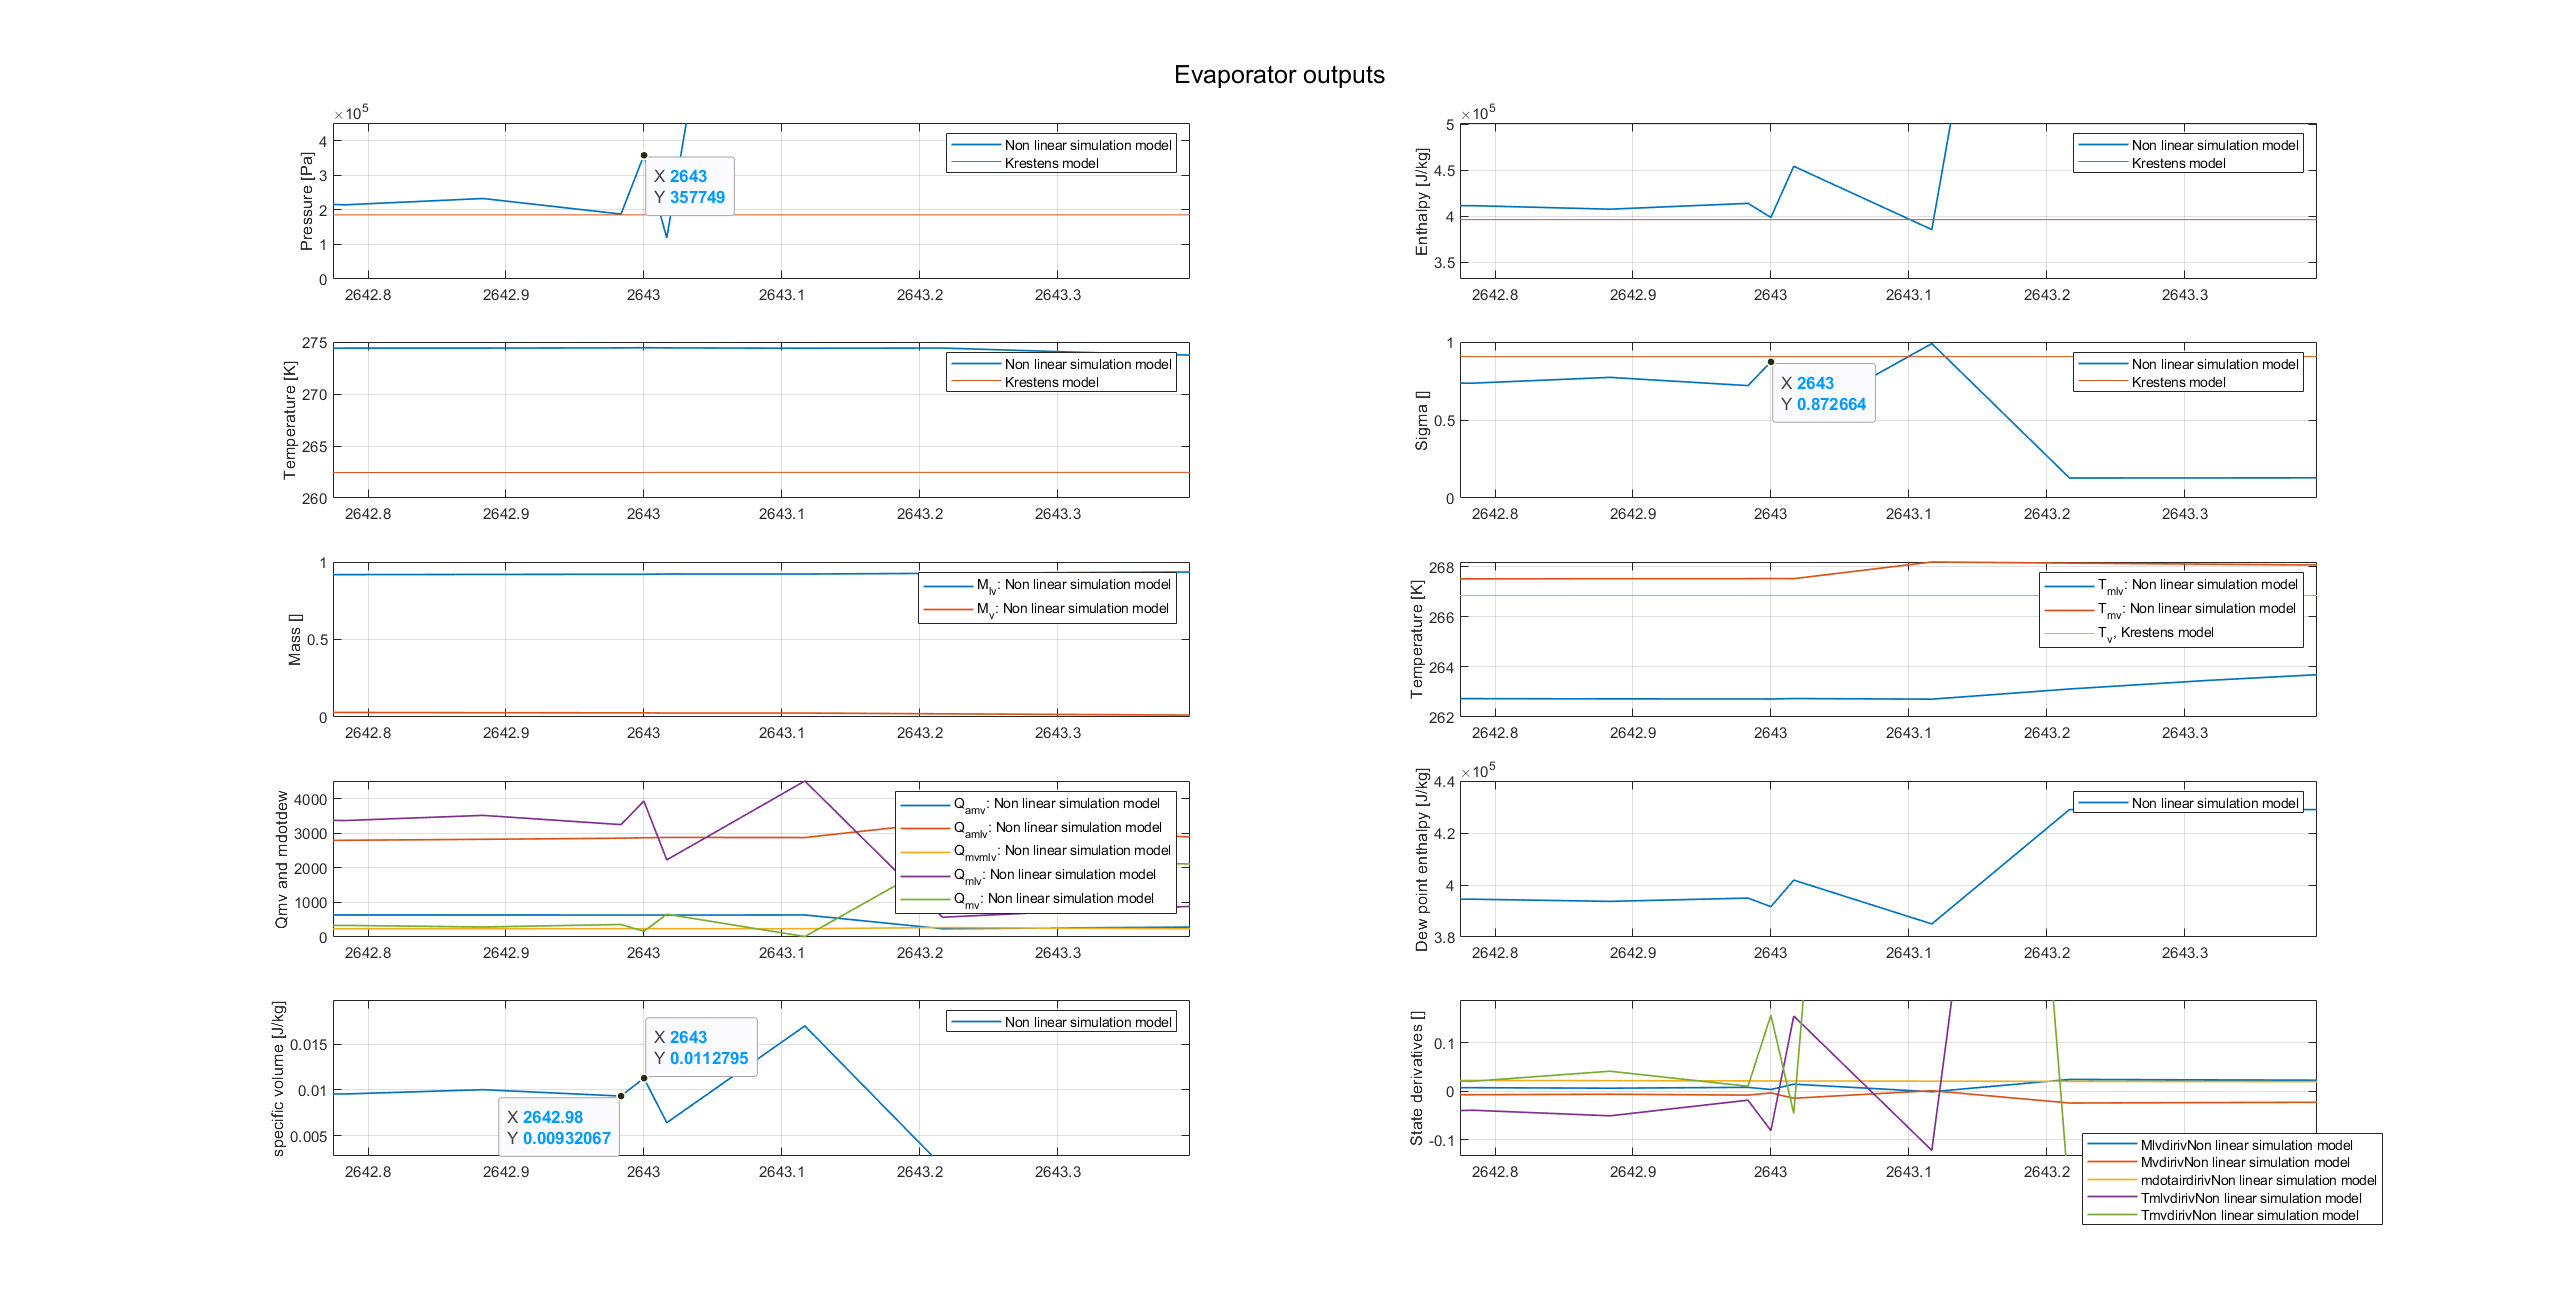
\includegraphics[width=2.1\textwidth]{Tests/Evapo_test1/plot_unstable_zoomed.png}
	\caption{Zoomed version of \cref{fig:evapotest_plot1}}
	\label{fig:evapotest_plot2}
\end{figure}
In \cref{fig:evapotest_plot2} is a zoom around time t = 2643 s where the simulation proves to start be unstable. From debugging, a sense of a positive feedback loop between look up table from the specific volume and the pressure was assumed. This was the root of the idea of setting $ p_{out} = p_{in} $

\begin{figure}[h]
	\centering
	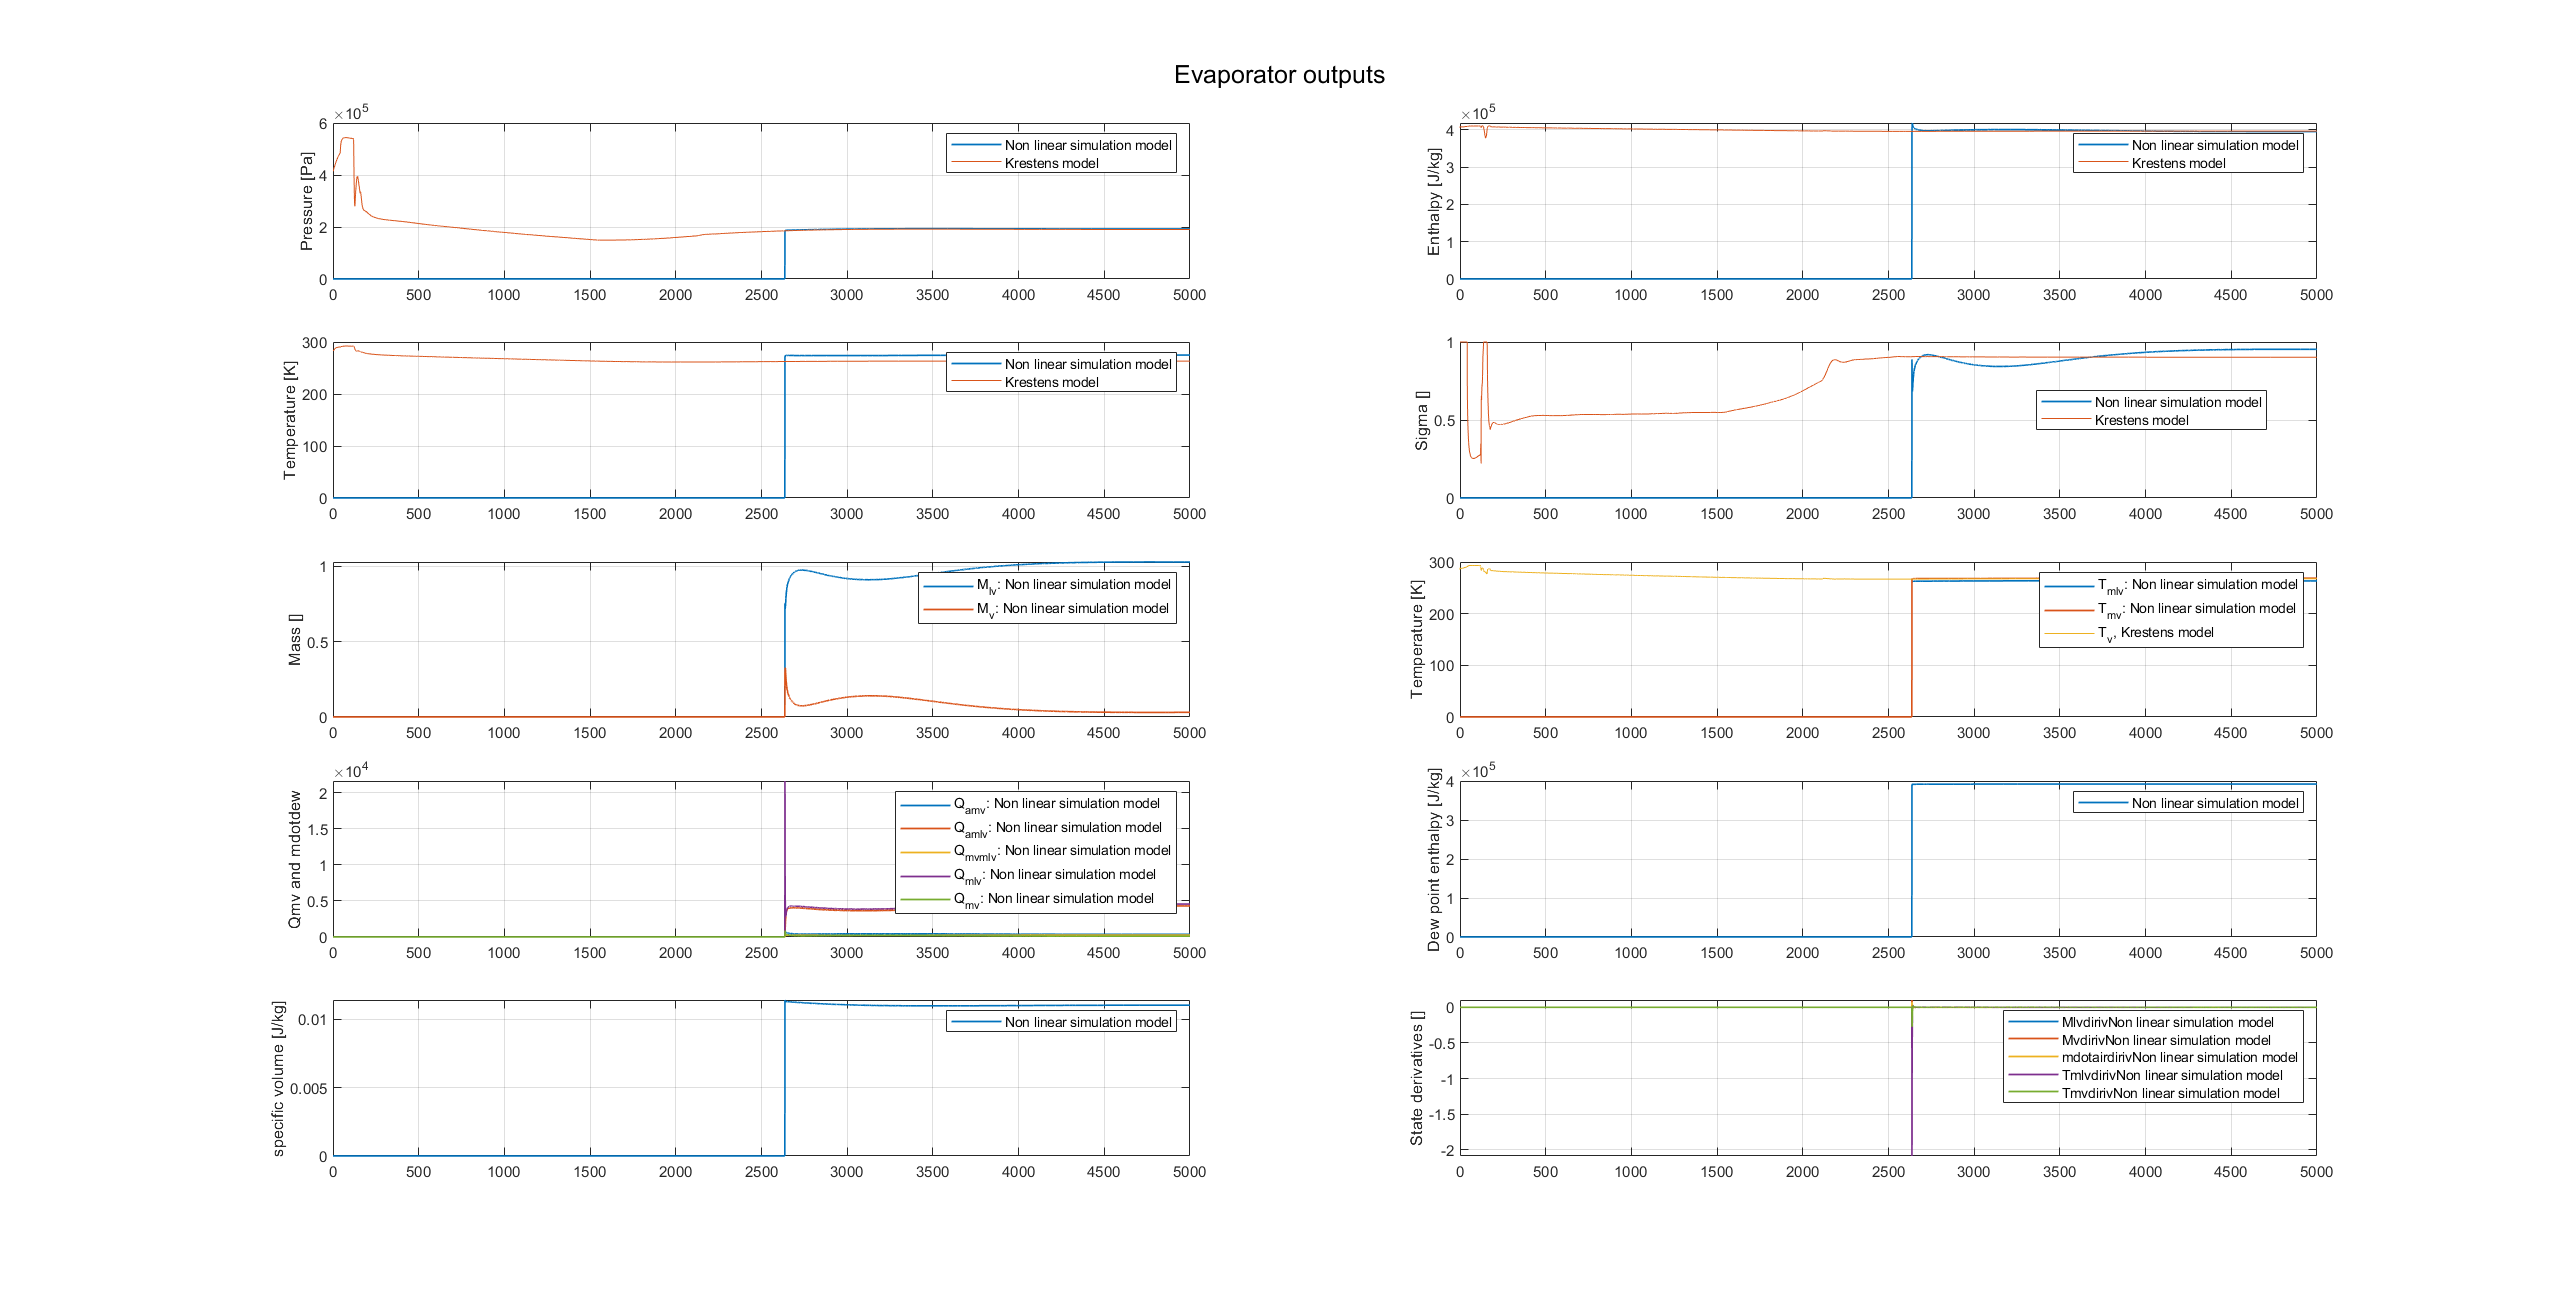
\includegraphics[width=2.1\textwidth]{Tests/Evapo_test1/plot_stable.png}
	\caption{Simulation with $ p_{out} = p_{in} $}
	\label{fig:evapotest_plot3}
\end{figure}

In \cref{fig:evapotest_plot3} where the output pressure is now equal to the input pressure, the behavior is much better, and for this reason we make the assumption that the output pressure is equal to the input pressure.

